%!Mode:: "TeX:UTF-8"
\section{B树及其变体}

\subsection{B树}
B树(B-tree)是一种树状数据结构,它能够存储数据、对其进行排序并允许以O(log n)的时间复杂度运行进行查找、顺序读取、插入和删除的数据结构。B树,概括来说是一个节点可以拥有多于2个子节点的二叉查找树。与自平衡二叉查找树不同,B树为系统最优化大块数据的读和写操作。B-tree算法减少定位记录时所经历的中间过程,从而加快存取速度。普遍运用在数据库和文件系统。

\begin{figure}[ht]
	\begin{center}
		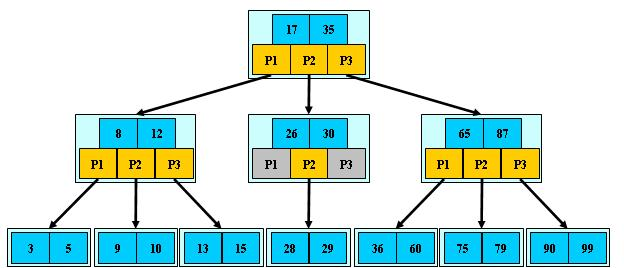
\includegraphics[keepaspectratio,width=0.6\paperwidth]{Pictures/BTree/BTreeBlogPicture.jpg}
	\caption{B树}
	\label{fig:BTreeBlogPicture}
	\end{center}
\end{figure}


根据Knuth的定义,m阶B树符合下列条件:
\begin{enumerate}
  \item 每个结点至多有m个子结点
  \item 除根结点外,非叶结点至少有$\lceil m/2 \rceil$ 个子结点
  \item 根结点至少有两个子结点,除非它是叶结点
  \item 非叶结点的关键词树比其子结点树少1
  \item 叶结点在同一层
\end{enumerate}
树的高度$h$(如果根结点为叶节点,高度为0)满足:$h \le \log_{\lceil m/2 \rceil}(\frac{n+1}{2})$。其中$n$为关键词数。

\subsection{B树操作}

\subsubsection{B树的搜索search(root, target)}
从root出发,对每个节点,找到大于或等于target关键字中最小的K[i],如果K[i]与target相等,则查找成功;否则在P[i]中递归搜索target,直到到达叶子节点,如仍未找到则说明关键字不在B树中,查找失败。
 
\subsubsection{B树的插入,insert(root, target)}
B树的插入需要沿着搜索的路径从root一直到叶节点,根据B树的规则,每个节点的关键字个数在[t-1, 2t-1]之间,故当target要加入到某个叶子时,如果该叶子节点已经有2t-1个关键字,则再加入target就违反了B树的定义,这时就需要对该叶子节点进行分裂,将叶子以中间节点为界,分成两个包含t-1个关键字的子节点,同时把中间节点提升到该叶子的父节点中,如果这样使得父节点的关键字个数超过2t-1,则要继续向上分裂,直到根节点,根节点的分裂会使得树加高一层。
 
上面的过程需要回溯,那么能否从根下降到叶节点后不回溯就能完成节点的插入呢?答案是肯定的,核心思想就是未雨绸缪,在下降的过程中,一旦遇到已满的节点(关键字个数为2t-1),就就对该节点进行分裂,这样就保证在叶子节点需要分裂时,其父节点一定是非满的,从而不需要再向上回溯。
 
\subsubsection{B树的删除,delete(root, target)}
在删除B树节点时,为了避免回溯,当遇到需要合并的节点时就立即执行合并,B树的删除算法如下:从root向叶子节点按照search规律遍历:
\begin{enumerate}
\item 如果target在叶节点x中,则直接从x中删除target,
情况(2)和(3)会保证当再叶子节点找到target时,肯定能借节点或合并成功而不会引起父节点的关键字个数少于t-1。
\item  如果target在分支节点x中:
	\begin{enumerate}
		\item 如果x的左分支节点y至少包含t个关键字,则找出y的最右的关键字prev,并替换target,并在y中递归删除prev。
		\item 如果x的右分支节点z至少包含t个关键字,则找出z的最左的关键字next,并替换target,并在z中递归删除next。
		\item 否则,如果y和z都只有t-1个关键字,则将targe与z合并到y中,使得y有2t-1个关键字,再从y中递归删除target。
	\end{enumerate}
\item 如果关键字不在分支节点x中,则必然在x的某个分支节点p[i]中,如果p[i]节点只有t-1个关键字:
	\begin{enumerate}
		\item 如果p[i-1]拥有至少t个关键字,则将x的某个关键字降至p[i]中,将p[i-1]的最大节点上升至x中。
		\item 如果p[i+1]拥有至少t个关键字,则将x个某个关键字降至p[i]中,将p[i+1]的最小关键字上升至x个。
		\item 如果p[i-1]与p[i+1]都拥有t-1个关键字,则将p[i]与其中一个兄弟合并,将x的一个关键字降至合并的节点中,成为中间关键字。
	\end{enumerate}
\end{enumerate}

\subsection{B+树和B*树数}
B+树是B树的变体,也是一种多路搜索树,其定义基本与B树同,除了:
\begin{enumerate}
  \item 非叶子结点的子树指针与关键字个数相同
  \item 非叶子结点的子树指针P[i],指向关键字值属于[K[i], K[i+1])的子树(B-树是开区间)
  \item 所有关键字都在叶子结点出现, 所有叶子结点增加一个链指针
\end{enumerate}
 B+的搜索与B-树也基本相同,区别是B+树只有达到叶子结点才命中(B-树可以在
非叶子结点命中),其性能也等价于在关键字全集做一次二分查找。

\begin{figure}[ht]
	\begin{center}
		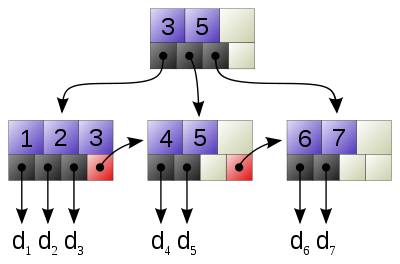
\includegraphics[keepaspectratio,width=0.6\paperwidth]{Pictures/BTree/BplusTree-wiki.png}
	\caption{B+树-维基百科图片}
	\label{fig:BplusTree-wiki}
	\end{center}
\end{figure}

B+树的特性:
\begin{enumerate}
  \item 所有关键字都出现在叶子结点的链表中(稠密索引),且链表中的关键字恰好是有序的
  \item 不可能在非叶子结点命中
  \item 非叶子结点相当于是叶子结点的索引(稀疏索引),叶子结点相当于是存储(关键字)数据的数据层
  \item 更适合文件索引系统
\end{enumerate}

\begin{figure}[ht]
	\begin{center}
		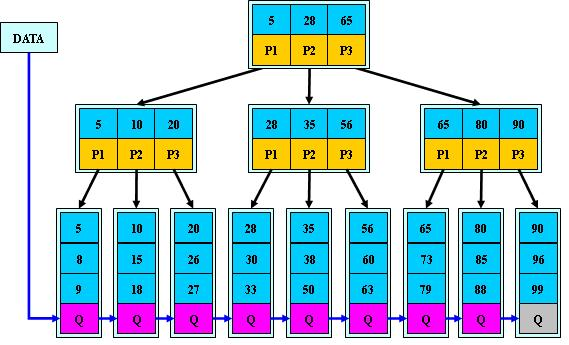
\includegraphics[keepaspectratio,width=0.6\paperwidth]{Pictures/BTree/BPlusTree.jpg}
	\caption{B+树}
	\label{fig:BplusTree}
	\end{center}
\end{figure}

Windows 文件系统NTFS 在 FAT 和 HPFS(高性能文件系统)的基础上作了一系列改进(如支持元数据)并且使用了更复杂的数据结构(B+树)以便于提升性能、改善可靠性并降低磁盘空间利用率。

B*树是B+树的变体,在B+树的非根和非叶子结点再增加指向兄弟的指针。
B*树定义了非叶子结点关键字个数至少为(2/3)*M,即块的最低使用率为2/3(代替B+树的1/2)。

B+树的分裂:当一个结点满时,分配一个新的结点,并将原结点中1/2的数据复制到新结点,最后在父结点中增加新结点的指针;B+树的分裂只影响原结点和父结点,而不会影响兄弟结点,所以它不需要指向兄弟的指针;

B*树的分裂:当一个结点满时,如果它的下一个兄弟结点未满,那么将一部分数据移到兄弟结点中,再在原结点插入关键字,最后修改父结点中兄弟结点的关键字(因为兄弟结点的关键字范围改变了);如果兄弟也满了,则在原结点与兄弟结点之间增加新结点,并各复制1/3的数据到新结点,最后在父结点增加新结点的指针;所以,B*树分配新结点的概率比B+树要低,空间使用率更高。

\clearpage









